\section{Descrizione del progetto}
Il progetto scritto in Scala prevede di andare ad affiancare, alla macchinetta del caffè gestita in ASMETA, un distributore automatico di bevande energetiche.
In particolar modo si è progettato un sistema con queste specifiche:
\begin{itemize}
	\item Ogni distributore automatico può essere impostato per funzionare in una lingua piuttosto che in un'altro: nel codice è gestitata solamente la possibilità di introdurre distirbutori automatici in lingua italiana e in lingua inglese.
	
	\item Questi distributori possono gestire le seguenti bevande energetiche (\textit{energy drink}):
	\begin{itemize}
		\item RedBull
		\item Monster
		\item Gatorade
		\item Italian
	\end{itemize}
	Ognuno di questi prodotti sarà caratterizzato dai seguenti campi descrittivi:
	\begin{itemize}
		\item prezzo
		\item volume (espresso in cl)
		\item data di scadenza
		\item insieme di tags, che permettono di esprimere le caratteristiche salienti di ognuno degli energy drink
	\end{itemize}
\end{itemize}

Ogni distributore andrà ad offrire le seguenti funzionalità:
\begin{itemize}
	\item Acquisto dei prodotti disponibili, regalando i prodotti scaduti: in particolare la macchinetta sarà in grado di fornire resto esatto al cliento (oppure tutta la somma di denaro inserita nel caso di prodotto scaduto).
	\item Mostrare l'elenco dei prodotti disponibili all'interno del distirbutore (identificato tramite ID), unitamente al numero di pezzi disponibili, come si vede in figura ~\ref{fig:AvailableProducts}.
	\begin{figure}[h]
		\centering
		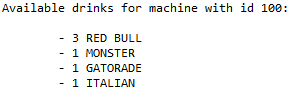
\includegraphics[width=0.3\textwidth]{Immagini/ShowVendingMachine.png}
		\caption{Prodotti disponibili}
		\label{fig:AvailableProducts}
	\end{figure}
	\item Possibilità di cercare un prodotto tramite tag, per poter così trovare l'energy drink più adatto ad ogni evenienza
	\item Aggiunta di energy drink all'interno del distributore: nello specifico, l'aggiunta di un nuovo prodotto, avviene all'interno di una struttra definita come un array di Queue (ovvero una matrice), che non fa altro che andare a riprodurre la fisionomia di un distirbutore reale.
\end{itemize}

\section{Gerarchia delle classi}
Nella applicazione realizzata sono stati realizzata due gerarchie facendo uso dei \textit{trait}: i trait in Scala corrispondono alle interfaccie in Java, ovvero permettono di definire la firma di ogni classe che ne implementa la struttura.
Nel nostro caso abbiamo due strutture gerarchiche, gestite tramite traits, mostrate con un grafo ad "albero", nelle seguenti immagini (figura ~\ref{fig:energyDrink} ~\ref{fig:vendingMachine}).
	\begin{figure}[h]
	\centering
	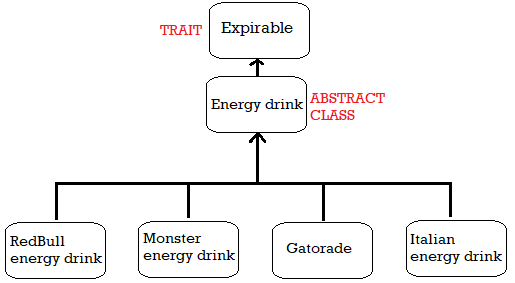
\includegraphics[width=0.8\textwidth]{Immagini/EnergyDrink.png}
	\caption{Energy drink}
	\label{fig:energyDrink}
\end{figure}
	\begin{figure}[h]
	\centering
	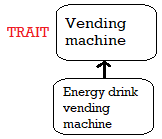
\includegraphics[width=0.8\textwidth]{Immagini/VendingMachine.png}
	\caption{Vending machine}
	\label{fig:vendingMachine}
\end{figure}

\section{Filter}
\section{Match}
